%! Author = Javier Mérida
%! Date = 2/12/2023

% Preamble
\documentclass[12pt]{report}
\parskip=\baselineskip
\setcounter{secnumdepth}{4}
% Packages
\usepackage[utf8]{inputenc}
\usepackage{graphicx}
\usepackage[smartEllipses]{markdown}
\usepackage{setspace}
\usepackage[table,xcdraw]{xcolor}
\usepackage{float}
\usepackage{url}
\usepackage[nottoc,notlot,notlof]{tocbibind}
\singlespacing
% Graphics
\graphicspath{ {images/} }
\floatplacement{figure}{H}
% Verbatim
\usepackage{framed,color,verbatim}
\usepackage{textcomp}
\usepackage[hidelinks]{hyperref}
\definecolor{shadecolor}{rgb}{.9, .9, .9}
\newenvironment{code}%
{\snugshade\verbatim}%
{\endverbatim\endsnugshade}
% title
\title{
    \vspace*{1cm}
    {
\includegraphics{lasalle-logo}}
    {Static Site Generator}\\
    {\large La Salle Campus Barcelona}\\
}
\author{Javier Mérida}
\date{12 02 2023}


% Document
\begin{document}

%%    \maketitle
%    \begin{titlepage}
%        \begin{center}
%%            \vspace*{1cm}
%            
\includegraphics[width=0.7\textwidth]{lasalle-logo}
%
%        \end{center}
%        \textbf{Static Site Generator}
%
%        \vspace{0.5cm}
%        An study of software design implementation following a minimalistic approach.
%
%        \vspace{1.5cm}
%
%        \textbf{Javier Baltazar Merida Morales}
%
%        \vfill
%
%        A thesis presented for the degree of\\
%        International Computer Engineering
%
%        \vspace{0.8cm}
%
%
%
%        Department Name\\
%        University Name\\
%        Country\\
%        Date
%
%    \end{titlepage}

    \chapter*{Abstract}\label{ch:ch:chapter}
    \section*{English}\label{sec:english}
    This project presents the development of a Static Site Generator. It will start with explanations and insights
    into what a Static Site Generator (SSG) is, and what is expected from it, with a study of the current state of
    the art, then evaluating what features will be considered for the development of a new one, based on what is
    currently available, and from this point a set of requirements will be built, using the Software Requirement
    Specification IEEE document guide, to establish what could be expected and/or required from it. After this, the
    document will explore a software design proposal, which may or not be followed in the implementation as further
    changes may be needed during development. Finally, it will reach some conclusions based on what has been achieved
    and whether the proposed approach was correct, or if there is any improvement that could be made or evaluated.

    \section*{Español}
    Este proyecto presenta el desarrollo de un Generador de Sitios Estáticos. Comenzará con explicaciones y
    perspectivas sobre qué es un Generador de Sitios Estático (SSG), qué se espera de él, con un estudio del estado
    actual del arte, para luego evaluar qué características se considerarán para el desarrollo de uno nuevo, basado
    en lo que está disponible actualmente, y a partir de este punto se construirá un conjunto de requisitos,
    utilizando la guía del documento de Especificación de requisitos de software IEEE, para establecer lo que se podría
    esperar y/o requerir del mismo. Después de esto, el documento explorará una propuesta de diseño de software, que
    puede seguirse o no en la implementación, ya que es posible que se necesiten más cambios durante el desarrollo.
    Finalmente, se llegará a algunas conclusiones en base a lo logrado, y si el enfoque propuesto fue correcto, o si
    existe alguna mejora que se pueda realizar o evaluar.

    \section*{Català}
    Aquest projecte presenta el desenvolupament d'un generador de llocs estàtics. Començarà amb explicacions i
    coneixements sobre què és un generador de llocs estàtics (SSG) i què se n'espera, amb un estudi de l'estat actual
    de la tècnica, i després avaluant quines característiques es tindran en compte per al desenvolupament d'un de nou
    . , basant-se en el que està disponible actualment, i a partir d'aquest punt es construirà un conjunt de
    requisits, utilitzant la guia de documents IEEE Software Requirement Specification, per establir què es podria
    esperar i/o requerir d'aquest nou model. Després d'això, el document explorarà una proposta de disseny de
    programari, que es pot seguir o no en la implementació, ja que poden ser necessaris més canvis durant el
    desenvolupament. Finalment, s'arriba a unes conclusions en funció del que s'ha aconseguit i de si l'enfocament
    proposat era correcte, o si hi ha alguna millora que es podria fer o avaluar.

    \tableofcontents

    %! Author = javif
%! Date = 9/13/2023


\chapter{Introduction}\label{ch:introduction}

Static site generators (SSGs)\cite{wikissg,cloudflare} have emerged as a crucial component of modern web development,
providing
numerous
benefits including speed, security, and ease of website administration. In recent years, their role in simplifying
the conversion of dynamic web content to static web pages has garnered widespread recognition. This thesis explores
the development of an SSG from inception to implementation, guided by a structured software development lifecycle
(SDLC), to contribute to the ever-changing landscape of SSGs.

This research is motivated by the constant evolution of web technologies and the rising demand for effective,
customizable, and user-friendly web development tools. This thesis aims to address the limitations and
inefficiencies
observed in current SSGs by systematically advancing through the stages of the software development life cycle (SDLC)
, including a review of the state of the art, defining rigorous requirements, proposing a robust design, implementing
the software, and evaluating the results.

This study commences with a comprehensive analysis of the current state of the art in static site generators. It will
evaluate the strengths, weaknesses, and compatibility of existing SSGs with contemporary web development
requirements\cite{khalid}
. This analysis not only provides a foundation for comprehending the extant landscape, but also identifies gaps and
improvement opportunities.

Following the evaluation, the research continues with the formulation of SRS (SRS Specifications). The SRS will
establish a precise list of requirements that this SSG must satisfy. These requirements will cover a broad
range of factors, including performance, security, extensibility, and user-friendliness, and will provide a detailed
road map for the development process.

The subsequent phase entails proposing a design that incorporates innovative solutions to resolve the identified
limitations and meet the specified requirements. During the design phase, architectural patterns, data models, and
the incorporation of modern web technologies will be considered in order to expand the SSG's capabilities.

After establishing a well-defined design, the thesis will proceed to the implementation phase. This phase will
involve the actual coding and development of the SSG, adhering to industry standards and software engineering
principles. Detailed documentation will accompany the implementation to assure transparency and reproducibility.

Finally, the thesis will conclude with a thorough examination of the results obtained from the enhanced SSG's
development. These results will be analyzed critically to determine how well the objectives and requirements were met
. Throughout the development lifecycle, any deviations, obstacles, and lessons learned will be highlighted, providing
valuable insights for future SSG enhancements and web development projects.

In conclusion, the objective of this thesis is to contribute to the field of web development by meticulously
enhancing the capabilities of static site generators. This research seeks to create a sophisticated and adaptable SSG
that aligns with the evolving needs of web developers, thereby enhancing the realm of static web content creation and
management.





    \chapter{Trying out popular SSGs}\label{ch:trying-out-popular-ssgs}

    The following SSGs has been chosen based on their popularity in order
    to be tried to gather information on what the basic features for SSG
    are.
    It's important to notice that these are being tried in a Linux environment
    (Linux inside Windows, thanks to WSL), installing them from scratch, using vim
    as text editor to minimize external tools assistance to have an unbiased appreciation
    of each one of them.

    \begin{itemize}
        \item NextJS (https://nextjs.org/)
        \item Hugo\cite{hugo}
        \item VuePress
        \item Eleventy
        \item Astro
    \end{itemize}

    % Trying NextJS
    \markdownInput{chapters/testing-ssgs/nextjs.md}

    % Trying Hugo
    \markdownInput{chapters/testing-ssgs/hugo.md}

    % Trying VuePress
    \markdownInput{chapters/testing-ssgs/vuepress.md}

    % Trying Eleventy
    \markdownInput{chapters/testing-ssgs/eleventy.md}

    % Trying Astro
    \markdownInput{chapters/testing-ssgs/astro.md}


    \section{Comparison Table}\label{sec:comparison-table}


    The following table outlines the features that has been considered as most important to take into account when
    considering static site generator.
    Note that the purpose of this document is not to benchmark any of these features,
    thus there is not a workload test to compare the performance of the explored SSGs. Instead, this is a simple
    exploration on what features are stand out in order to consider as requisites to build a new SSG.


    Also, it is important to note that the lack or the presence of any of these characteristic do not make any SSG
    better
    than others, as each one of them are made for a specific purpose and shine in terms of addressing the obstacle
    they are meant to\cite{khalid}.
    In fact, this section must be taken as an exploration of requisites to be taken into account.


    % Please add the following required packages to your document preamble:
% \usepackage[table,xcdraw]{xcolor}
% If you use beamer only pass "xcolor=table" option, i.e. \documentclass[xcolor=table]{beamer}
    \begin{table}[H]
        \begin{tabular}{|
                >{\columncolor[HTML]{EFEFEF}}c |c|c|c|c|c|}
            \hline
            \cellcolor[HTML]{C0C0C0} & \cellcolor[HTML]{EFEFEF}NextJS & \cellcolor[HTML]{EFEFEF}Hugo &
            \cellcolor[HTML]{EFEFEF}VuePress & \cellcolor[HTML]{EFEFEF}Eleventy & \cellcolor[HTML]{EFEFEF}Astro \\
            \hline
            \textbf{Easy to use} & Yes & Yes & No
            & Yes & Yes \\ \hline
            \textbf{Flexible} & No & No & No
            & Yes & Yes \\ \hline
            \textbf{Strict structure} & No & Yes & No
            & No & No \\ \hline
            \textbf{Template system} & No & Yes & No
            & Yes & Yes \\ \hline
            \textbf{Themes} & No & Yes & No
            & Yes & Yes \\ \hline
            \textbf{Performance oriented} & Yes & Yes & NA
            & Yes & Yes \\ \hline
            \textbf{Framework dependant} & Yes & No & Yes
            & No & No \\ \hline
            \textbf{Easy to install} & Yes* & Yes & Yes*
            & Yes* & Yes* \\ \hline
            \textbf{File-based routing} & Yes & Yes & NA
            & Yes & Yes \\ \hline
        \end{tabular}\label{tab:table}
    \end{table}


    Note*: The installation difficulty is strickly dependant of NodeJS and how `npm` addresses any missing dependency,
    which can be (sometimes) a painful issue to solve.

    % SRS


    \chapter{Software requirements specifications}\label{ch:software-requirements-specifications}

    % SRS Introduction.
    %\markdownInput{chapters/requirements/introduction.md}
    %! Author = javif
%! Date = 9/13/2023


\chapter{Introduction}\label{ch:introduction}

Static site generators (SSGs)\cite{wikissg,cloudflare} have emerged as a crucial component of modern web development,
providing
numerous
benefits including speed, security, and ease of website administration. In recent years, their role in simplifying
the conversion of dynamic web content to static web pages has garnered widespread recognition. This thesis explores
the development of an SSG from inception to implementation, guided by a structured software development lifecycle
(SDLC), to contribute to the ever-changing landscape of SSGs.

This research is motivated by the constant evolution of web technologies and the rising demand for effective,
customizable, and user-friendly web development tools. This thesis aims to address the limitations and
inefficiencies
observed in current SSGs by systematically advancing through the stages of the software development life cycle (SDLC)
, including a review of the state of the art, defining rigorous requirements, proposing a robust design, implementing
the software, and evaluating the results.

This study commences with a comprehensive analysis of the current state of the art in static site generators. It will
evaluate the strengths, weaknesses, and compatibility of existing SSGs with contemporary web development
requirements\cite{khalid}
. This analysis not only provides a foundation for comprehending the extant landscape, but also identifies gaps and
improvement opportunities.

Following the evaluation, the research continues with the formulation of SRS (SRS Specifications). The SRS will
establish a precise list of requirements that this SSG must satisfy. These requirements will cover a broad
range of factors, including performance, security, extensibility, and user-friendliness, and will provide a detailed
road map for the development process.

The subsequent phase entails proposing a design that incorporates innovative solutions to resolve the identified
limitations and meet the specified requirements. During the design phase, architectural patterns, data models, and
the incorporation of modern web technologies will be considered in order to expand the SSG's capabilities.

After establishing a well-defined design, the thesis will proceed to the implementation phase. This phase will
involve the actual coding and development of the SSG, adhering to industry standards and software engineering
principles. Detailed documentation will accompany the implementation to assure transparency and reproducibility.

Finally, the thesis will conclude with a thorough examination of the results obtained from the enhanced SSG's
development. These results will be analyzed critically to determine how well the objectives and requirements were met
. Throughout the development lifecycle, any deviations, obstacles, and lessons learned will be highlighted, providing
valuable insights for future SSG enhancements and web development projects.

In conclusion, the objective of this thesis is to contribute to the field of web development by meticulously
enhancing the capabilities of static site generators. This research seeks to create a sophisticated and adaptable SSG
that aligns with the evolving needs of web developers, thereby enhancing the realm of static web content creation and
management.




    % SRS Overall description
    %\markdownInput{chapters/requirements/description.md}
    %! Author = javif
%! Date = 9/14/2023

\subsection{Overall description}\label{subsec:overall-description}

\subsubsection{Product perspective}\label{subsubsec:product-perspective}

\texttt{VaGo} is not the first SSG, nor does it claim to be unique or
break any industry standards. Instead, it focuses on providing a simple
interface for both the content creator (intended to work primarily in
markdown files) and the theme author to create and style websites (meant
to provide default styles while deciding editable parameters).

In this regard, it is very similar to, and in fact inspired by,
HuGo\cite{hugo}\cite{wikihugo}, another SSG written in the Go programming language.
Despite this, \texttt{VaGo} attempts to adopt a comparable theming
methodology while incorporating simplified modification capabilities.
This would enable prospective users to reuse and personalize
pre-existing themes without the need to delve into CSS files.
Furthermore, the system in question lacks a focus on performance and
does not aim to rival HuGo in this regard. HuGo is renowned for its
exceptional performance in generating and delivering static content.

In contrast to NextJS and VuePress\cite{vuepress}, which utilize React and Vue,
respectively, for component creation and usage, \texttt{VaGo} does not
employ a framework-based component system. In contrast, \texttt{VaGo}
restricts itself to utilizing only native HTML, JS, and CSS. However,
this does not necessarily preclude the platform from leveraging Go to
facilitate or circumvent boilerplate when converting content into the
aforementioned web technologies.

Additionally, the product is not intended to incorporate any reactive
techniques or external frontend frameworks in order to achieve similar
results. The entirety of the content is intended to be loaded and
produced on the server side\cite{sunssr}, with no additional features on the client
side, unless the user chooses to incorporate them using JavaScript. It
is noteworthy that the utilization of opinionated simplicity fulfills
the objective of facilitating content creation for users, as they are
not required to attend to such particulars. However, this approach is
accompanied by the disadvantage of restricted customization options.

Furthermore, it should be noted that initially, there will be no
available modules or tools for integration with this particular static
site generator (SSG) framework, unlike other frameworks such as Astro.
This is because the development of such modules is not a primary focus
of the framework's feature development. Additionally, there are no plans
to introduce a module customization feature, as outlined in the
accompanying documentation.

Ultimately, it is imperative that end-users possess the capability to
engage with the product through a straightforward Command Line Interface
(CLI) to produce static content and subsequently distribute it online,
with minimal parameters and concealed features. Ideally, the system
should be designed to facilitate user comprehension and operation
without necessitating the perusal of a cumbersome 30-page manual replete
with convoluted directives and extraneous verbiage. Thus, it is apparent
that a minimal number of commands, typically two or three, accompanied
by fundamental parameters such as port, testing mode, and designated
source folder, should suffice to initiate the task at hand.

\subsubsection{Product functions}\label{subsubsec:product-functions}

This Static Site Generator's primary objective is to convert markdown
files' text to plain HTML, mapping the markup elements to understandable
web elements in order to maintain the Web Standards' accessibility\cite{accwai}\cite{basismoz}.

However, it should also be able to offer a theme system built on CSS
files that gives the HTML elements styling. This will be made possible
by also producing CSS with a set of additional parameters that follow a
pre-established structure and should be simple to alter using Go
variables.

Last but not least, \texttt{VaGo} will have a brief set of parameters to
enable communication with the user via CLI, to enable them to create
static content (translation of markdown to HTML with the addition of a
theme via CSS), and to serve content via a particular port. A set of
features for exporting and importing themes from authors whose works are
shared online and/or in repositories may be added in the future.

\subsubsection{User characteristics}\label{subsubsec:user-characteristics}

\texttt{VaGo} is designed to be utilized by individuals possessing a
basic understanding of web development and terminal operations. However,
this does not necessarily demand that they must hold a degree in
Computer Science in order to effectively employ the system. The primary
objective of the system is to facilitate ease of use for individuals
with limited knowledge of computer technologies, including academic
scientists seeking to disseminate their knowledge, blog posts, papers,
and ideas on the internet, without requiring extensive knowledge of web
technologies.

Therefore, a computer-based academic background is not needed for this
system to be used, as long as there is a bit of knowledge about markdown
and how to use a terminal, it should be entirely enough. Henceforth,
individuals possessing a greater depth of knowledge would be capable of
executing more intricate undertakings by leveraging the available
adaptability while adhering to the prescribed limitations.

\subsubsection{Constraints}\label{subsubsec:constraints}

Considering that \texttt{VaGo} is programmed using the Go language,
which inherently supports cross-platform functionality, the development
efforts will be concentrated solely on Linux to streamline the
implementation of CLI features and circumvent potential complications
arising from newline interpretation and other cross-platform
limitations.

In addition, the system does not account for security considerations
related to delivering content over the internet, and therefore it cannot
guarantee any level of safety in this regard beyond what is already
provided by the Go programming language.

However, while there exist fundamental performance considerations for
its implementation, it neither guarantees nor rivals other frameworks
with respect to performance, velocity, or optimal resource utilization.

Consequently, the implementation and development of \texttt{VaGo} will
primarily rely on the pre-existing features of the language. As such, it
is not anticipated that \texttt{VaGo} will establish its own mechanisms
for managing HTTP requests, signaling protocols for handshaking, thread
management through Go routines, or other hardware-related dependencies
and controls for the host computer. Therefore, any inherent limitations
within the Go programming language will inevitably impact the system,
and no resources will be allocated towards attempting to circumvent
them.

\subsubsection{Assumptions and
dependencies}\label{subsubsec:assumptions-and-dependencies}

The complete functioning of the SSG is contingent upon the availability
of the Linux operating system for its execution. Furthermore, the
accurate interpretation of Markdown files is contingent upon the
existence of well-crafted documents, without which complications may
arise.

In addition, it is anticipated that any additional alterations to the
styling will be heavily reliant on one's proficiency in CSS.
Consequently, it is imperative that these modifications are accurate, as
the system will not undertake any measures to verify the correctness of
CSS files.

Moreover, in the event that the system is utilized for the purpose of
delivering and sharing files, notably static content, it is anticipated
that an internet connection will be accessible to facilitate
communication with client-side requests. It is noteworthy that there
will be no verification implemented on this communication, nor will
there be any specific error handling beyond what is inherent to the
language.

Alternatively, the system's potential expansion could be facilitated
through the utilization of native JavaScript, thereby introducing
interactive elements to the otherwise static content. However, it is
important to note that \texttt{VaGo} does not assume responsibility for
this aspect, and any modifications or augmentations are solely at the
discretion of the user.

Vago's proper usage and functioning necessitate a collection of
dependencies, including the Go HTTP module for internet traffic serving.
These dependencies are managed by the Go modules import mechanism.
Therefore, it's assumed that these dependencies are available in the
host machine to be used by the system, and a default error message for
the missing dependencies will be thrown in case these are not installed,
without fancy or added complexity.

\subsubsection{Apportioning of
requirements}\label{subsubsec:apportioning-of-requirements}

It is possible that in the future, the system may incorporate
supplementary functionalities for the development and utilization of Web
Components using conventional web technologies, devoid of any
frameworks. The inclusion of these components may introduce an
additional level of intricacy and consequently enhance adaptability in
generating unique elements and segregating styling. This could
potentially enable an approach akin to the Astro islands architecture,
featuring isolated CSS. However, a noteworthy advantage lies in the
utilization of solely standard technologies, thereby eliminating the
need for supplementary tooling or increased size to support the same.

In addition, \texttt{VaGo} has the potential to provide fundamental
capabilities for generating said components, by eliminating the
redundant code required to construct a rudimentary web component, and
furnishing a platform to associate specific functionalities to them,
without necessitating extensive knowledge of JavaScript coding to
achieve the same outcome. It is possible to write the components using
Go language with the aid of VaGo, and subsequently interpret and convert
them into JavaScript for the purpose of generating the Web Component.

Nonetheless, it should be noted that the act of translating may result
in a loss of flexibility due to its dependence on the system's
interpretation. Despite this, it may prove to be a suitable solution for
a majority of component types commonly found in the industry. To gain a
deeper understanding of the current state of such technologies and their
relevance to existing needs, a comprehensive analysis of popular
frameworks and their approaches is necessary.


    % SRS Specific requirements.
%    \markdownInput{chapters/requirements/requirements.md}
    %! Author = javif
%! Date = 9/14/2023

\section{Specific requirements}\label{sec:specific-requirements}

\subsection{External interfaces}\label{subsec:external-interfaces}

Users will be able to interact with the system using CLI commands\cite{wikicli} to
carry out simple operations that are built into the system. Here, two
fundamental commands should be noted:

\begin{itemize}
    \item
    \texttt{Build}: To parse and generate HTML content from markdown files.
    \item
    \texttt{Serve}: To serve and share content via a specific port.
\end{itemize}

Additionally, the system ought to alert the user any time a command it
has issued contains an error because it is possible for them to
accidentally type the wrong command or misspell any of these. (using
buidl instead of build). Notably, unlike other systems, it will lack a
recommendation system to offer hints of similar words that are actually
interpreted as to assist the user in finding alternative commands, even
though it will inform the user about the existence of an error that
prevented the system from performing the required task.

\subsubsection{Build}\label{subsubsec:build}

The task at hand involves the conversion of Markdown files\cite{wikimd} into
web-based content, specifically in the form of HTML\cite{htmlmoz}, JS\cite{jsmoz}, and CSS\cite{cssmoz}.

The program is designed to utilize the Command Line Interface (CLI) as
an input mechanism, whereby it recognizes the command name to execute
its designated task. Its output function involves generating the HTML
and CSS content into an \texttt{out} folder, in accordance with the
pre-existing Markdown files. It is noteworthy that each MD file ought to
generate an individual page to allow for the adaptability of
transforming every file into a distinct output for the website.

Throughout the translation process, it is imperative that the user is
kept informed of its progress. In the event of any errors, the system
should prompt error messages to ensure the accuracy of the MD files,
while simultaneously verifying that all necessary parameters for content
and styling have been provided. Upon completion, the system should
explicitly indicate the out folder path to the user.

Therefore, it should use the following format for each of the steps
considered for the translation and building process: {[}Date{]}{[}Page
Name{]}: Step, where each one of these detail token corresponds to:

\begin{itemize}
    \item
    Date: Specific date and time using the ISO 8601 format\cite{wikiiso} without specifying
    the timezone as \texttt{VaGo} will limit itself to use the same
    timezone from the host machine. For instance: \emph{2023-04-09T14:
    22:05} should be used to represent the year 2023, month April (04),
    day 09 at 14 hours, 22 minutes and 05 seconds.
    \item
    Page Name: To specify the exact page name for the URL that takes to
    that specific page, which is the same as the MD file name.
    \item
    Step: To specify the building step it's currently on, whether it is
    identifying the MD tokens\cite{schutze2008introduction, wikilexical}, performing translation to HTML and/or
    obtaining the parameters set for the theming and styling of the given
    page.
\end{itemize}

On the other hand, additional parameters can be added to the command for
specific output capabilities. For instance, \texttt{no-log} should be
using to omitting logging (no prompt message for every building process
step) except for error and finalization message. Also, \texttt{no-time}
should be used to omit the timestamp from the steps, prompting a message
with the following structure: \emph{{[}Page name{]}:Step}, with the
purpose of avoiding overloading logs and make them easier to read.

\subsubsection{Serve}\label{subsubsec:serve}

The second command serves the purpose of keep the system continuously
executing, hence no accepting other commands in the meantime, in order
to open a port and send the already built files (by means of the
previous command, \texttt{build}) via HTTP\cite{gourley2002http}.

It is important to note that this command will exclusively serve content
available in the \texttt{out} folder, therefore if the previous command
hasn't been run, or if there are no files in this folder, then it won't
be able to serve any content at all. Because of it, it is required that
the user must first build content in order to then serve it.

Moreover, in addition to the behavior noted above, it must output logs
to inform the user of the current status of the serving process,
starting by indicating as soon as it starts reading content and
initiating listening for requests, while also informing of any issue
that may occur by prompting error messages.

Once it starts listening for requests, it should inform of any incoming
request/response using the following format: {[}Date{]}: Sending
        {[}Page{]} to {[}requester IP{]}, where each one of these token
corresponds to:

\begin{itemize}
    \item
    Date: Same as the one outlined for \texttt{build} command, using the
    ISO 8601 format without timezone.
    \item
    Page: Page name as stated in the MD filename.
    \item
    Requester IP: Specific IP address of the incoming IP.
\end{itemize}

Additionally, an extra (optional) parameter can be provided to outline
the specific port the system should open to listen for requests, instead
of the default one.

\subsection{Functions}\label{subsec:functions}

The following provides a more in-depth explanation of the functional
areas, including full requirements.

\subsubsection{Generate page}\label{subsubsec:generate-page}

\paragraph{Description and priority}\label{par:description-and-priority}

The task at hand involves generating a page document through the process
of translating the contents of a Markdown file into HTML. This requires
the utilization of appropriate tags to accurately map the entities
present within each Markdown block. Priority: HIGH.

\paragraph{Stimulus/Response
sequences}\label{par:stimulusresponse-sequences}

Stimulus: This feature must obtain the markdown files from a
\texttt{source} folder.

Response: Translate or generate a corresponding HTML file for each one
of these MD files, outputting the result pages into an \texttt{out}
folder.

\paragraph{Functional requirements}\label{par:functional-requirements}

\textbf{REQ-1}: The MD blocks must be interpreted and translated to HTML
tags to generate a page accordingly to what the user has described
initially. It should, at least, implement the following elements to
ensure a fully accessible page as per best practices for web standards\cite{accmoz}:

\begin{itemize}
    \item
    Heading level 1 (\texttt{\#}): Heading 1
    (\texttt{\textless{}h1\textgreater{}\textless{}/h1\textgreater{}}).
    \item
    Heading level 2 (\texttt{\#\#}): Heading 2
    (\texttt{\textless{}h2\textgreater{}\textless{}/h2\textgreater{}}).
    \item
    Heading level 3 (\texttt{\#\#\#}): Heading 3
    (\texttt{\textless{}h3\textgreater{}\textless{}/h3\textgreater{}}).
    \item
    Heading level 4 (\texttt{\#\#\#\#}): Heading 4
    (\texttt{\textless{}h4\textgreater{}\textless{}/h4\textgreater{}}).
    \item
    Heading level 5 (\texttt{\#\#\#\#\#}): Heading 5
    (\texttt{\textless{}h5\textgreater{}\textless{}/h5\textgreater{}}).
    \item
    Heading level 6 (\texttt{\#\#\#\#\#\#}): Heading 6
    (\texttt{\textless{}h6\textgreater{}\textless{}/h6\textgreater{}}).
    \item
    Text: Paragraph
    (\texttt{\textless{}p\textgreater{}\textless{}/p\textgreater{}}).
    \item
    Bold text (\texttt{**text**}): Strong
    (\texttt{\textless{}strong\textgreater{}\textless{}/strong\textgreater{}}).
    \item
    Italic text (\texttt{\_text\_}): Emphasis
    (\texttt{\textless{}em\textgreater{}\textless{}/em\textgreater{}}).
    \item
    Blockquote (\texttt{\textgreater{}}): Blockquote
    (\texttt{\textless{}blockquote\textgreater{}\textless{}/blockquote\textgreater{}}).
    \item
    Unordered list (\texttt{-}): Unordered list
    (\texttt{\textless{}ul\textgreater{}\textless{}/ul\textgreater{}})
    surrounding list items
    (\texttt{\textless{}li\textgreater{}\textless{}/li\textgreater{}}).
    \item
    Ordered list (\texttt{1.}, \texttt{2.}, \texttt{3.}, and so): Ordered
    list
    (\texttt{\textless{}ol\textgreater{}\textless{}/ol\textgreater{}})
    surrounding list items
    (\texttt{\textless{}li\textgreater{}\textless{}/li\textgreater{}}).
    \item
    Code (\texttt{\textasciigrave{}\textasciigrave{}}): Code
    (\texttt{\textless{}code\textgreater{}\textless{}/code\textgreater{}}).
    \item
    Fenced code block
    (\texttt{\textasciigrave{}\textasciigrave{}\textasciigrave{}\ \textasciigrave{}\textasciigrave{}\textasciigrave{}}):
    Preformatted text
    (\texttt{\textless{}pre\textgreater{}\textless{}/pre\textgreater{}})
    surrounding a code block
    (\texttt{\textless{}code\textgreater{}\textless{}/code\textgreater{}}).
    \item
    Link (\texttt{{[}text{]}(URL)}): Anchor tag along with the hyperlink
    attribute
    (\texttt{\textless{}a\ href="URL"\textgreater{}text\textless{}/a\textgreater{}}).
    \item
    Image (\texttt{!{[}Alt\ text{]}(URL)}): Image tag along with alt text
    and source attributes
    (\texttt{\textless{}img\ alt="Alt\ text"\ src="URL"\textgreater{}\textless{}/img\textgreater{}}).
\end{itemize}

\textbf{REQ-2}: It must verify whenever there is an input error or
incorrect usage of the MD blocks, and thereby let the user know about
these via error messages and halt the translation process immediately.

\textbf{REQ-3}: Each generated page will have the same file name as the
input MD file.

\subsubsection{Theme styling creation and
customization}\label{subsubsec:theme-styling-creation-and-customization}

\paragraph{Description and
priority}\label{par:description-and-priority-1}

This feature is responsible for enabling the construction of a
customizable theme for styling purposes. As long as the author (the
theme creator) enhances these capabilities via exposed variables, it
will manage CSS files that will provide styles to the pages and provide
functionalities to perform tweaks and changes to the theme. Therefore,
subsequent users of the same theme would be able to make certain
modifications to suit their needs, while retaining the already provided
set of opinionated styles. Priority: MEDIUM.

\paragraph{Stimulus/Response
sequences}\label{par:stimulusresponse-sequences-1}

Stimulus: Single or multiple files with preprocessed CSS attributes that
will receive the values of the exposed variables to be processed into a
final CSS file. Notice that the format of this file is not strictly CSS
as it should be noted that it is waiting for the building stage to add
the variables, therefore it's suggested to use a temporal file name
adding \texttt{.go.css} to differentiate it from its final version.

Response: Once processed, the file or set of files will be merged into a
single one, following an established structure and adding the exposed
variables via Go.

Stimulus: Authored parameters in the form of Go variables. There is also
the possibility of exposing such variables via YAML\cite{wikiyaml} or JSON\cite{wikijson} format, to
avoid overwriting Go code.

Response: The parameters are added to the final CSS file.

\textbf{REQ-1}: The exposed parameters should be added within the
preprocessed style file using the pattern
\texttt{\$\{{[}variable\ name{]}\}} in the same place where it will be
replaced.

\textbf{REQ-2}: These variables are then added or modified within a
specific Go module specifically designed for this purpose. Thereby, the
author will be able to expose these in this file, and add a default
value in case the user decides to not change anything. It should be
noted that the system won't take care of the compilation or verification
of the CSS file, hence it is completely up to the author to verify
whether it is correctly built.

\textbf{REQ-3}: Multiple style files could be added together in a single
final one, providing the author the flexibility to split them into
different modules for readability and maintainability purposes, thus
these must be specified in a Go module specifically designed for this
purpose, or within a main preprocessed style file using the nomenclature
\texttt{\$\{\#module:\ {[}file\ name{]}\}}.

\textbf{REQ-4}: The system must verify and prompt a clear error message
when there is a theme variable that has not been set. More specifically,
it should display a message using the following structure:
``\emph{Error: {[}variable name{]} has not been initialized.}'', where
the variable name will be replaced with the specific variable missing
its initialization.

\subsubsection{Templating}\label{subsubsec:templating}

\paragraph{Description and
priority}\label{par:description-and-priority-2}

The proposed system will incorporate a functionality that enables the
establishment of a predetermined framework or outline, in addition to
the primary template, for organizing the content into web pages. It is
noteworthy that the utilization of Go language's templating capabilities
is integral to the handling of this task. However, the system must
furnish a mechanism for retrieving the primary information components
from the markdown files. This will enable easy recognition and
referencing of said components in the template, thereby facilitating
customization. Priority: MEDIUM.

\paragraph{Stimulus/Response
sequences}\label{par:stimulusresponse-sequences-2}

Stimulus: Single or multiple HTML files with Go templating variables to
be filled with, from which the user can decide to use custom variables
(from custom Go code) or the main, already provided variables from the
markdown file components (headings, text, bold, italic, lists, etc).

Response: When built, a final HTML file should be prompted with the
provided content via markdown files and following the provided structure
or skeleton as in the template.

\paragraph{Functional requirements}\label{par:functional-requirements-1}

\textbf{REQ-1}: The processed format must follow the established
skeleton from the template. If there is no provided template, the system
must use a base one already provided with the generator.

\textbf{REQ-2}: Each markdown component should be accessible via Go
variables following this naming convention:

\begin{itemize}
    \item
    Heading level 1 (\texttt{\#}): \texttt{H1}
    \item
    Heading level 2 (\texttt{\#\#}): \texttt{H2}.
    \item
    Heading level 3 (\texttt{\#\#\#}): \texttt{H3}.
    \item
    Heading level 4 (\texttt{\#\#\#\#}): \texttt{H4}.
    \item
    Heading level 5 (\texttt{\#\#\#\#\#}): \texttt{H5}.
    \item
    Heading level 6 (\texttt{\#\#\#\#\#\#}): \texttt{H6}.
    \item
    Text: \texttt{B}.
    \item
    Bold text (\texttt{**text**}): \texttt{Strong}.
    \item
    Italic text (\texttt{\_text\_}): \texttt{Em}.
    \item
    Blockquote (\texttt{\textgreater{}}): \texttt{Blockquote}.
    \item
    Unordered list (\texttt{-}): \texttt{Ul}.
    \item
    Ordered list (\texttt{1.}, \texttt{2.}, \texttt{3.}, and so):
    \texttt{Ol}.
    \item
    Code (\texttt{\textasciigrave{}\textasciigrave{}}): \texttt{Code}.
    \item
    Fenced code block
    (\texttt{\textasciigrave{}\textasciigrave{}\textasciigrave{}\ \textasciigrave{}\textasciigrave{}\textasciigrave{}}):
    \texttt{Pre}.
    \item
    Link (\texttt{{[}text{]}(URL)}): \texttt{A}, \texttt{A.URL}.
    \item
    Image (\texttt{!{[}Alt\ text{]}(URL)}): \texttt{Img},
    \texttt{Img.Alt}, \texttt{Img.Src}.
\end{itemize}

It is important to note that the naming convention and HTML elements are
identical. This is intentional, as it should direct the user to the
correct element the component should be used in, so as to maintain best
practices for web accessibility and search engine optimization, avoiding
the use of meaningless \texttt{div} tags everywhere.

\subsubsection{Configuration files}\label{subsubsec:configuration-files}

\paragraph{Description and
priority}\label{par:description-and-priority-3}

Through the configuration files the user will be able to set up certain
parameters that will change the way the system works to adapt it to
given needs and setup, such as determine specific input and output
folders, theme name, template file name, author information (name,
website name, creation date), and others. It's worth noting that these
configuration files are not strictly necessary as the system must
initiate with a set of given default parameters, which can be
overwritten for extended customization. Priority: LOW.

\paragraph{Stimulus/Response
sequences}\label{par:stimulusresponse-sequences-3}

Stimulus: A Go\cite{donovan2015go}, JSON\cite{wikijson} or YAML\cite{wikiyaml} file with the set of parameters to be read
from, so the system can use them as variables for its configuration. The
type of file to be used will depend on the development time, as reading
directly from a Go file or module it's easier and faster to implement
than a JSON or YAML file, as it requires a parsing step first.

Response: The system will produce and/or build the static content
following these parameters accordingly.

\paragraph{Functional requirements}\label{par:functional-requirements-2}

\emph{REQ-1}: The system will use a set of default values if the
configuration files are not provided/changed, thus it is not strictly
needed for the system to work properly.

\emph{REQ-2}: The following configuration files must be scanned (found
via specific filename) and used for its respective purpose: Theme config
(\texttt{theme.*}, ) to specify styling parameters as well as the theme
name, template config (` layout.\emph{) to specify the files entries for
templating, main configuration (main.}) for the main parameters for
VaGo. File extension to be decided depending on development time as
noted on previous point.

\emph{REQ-3}: For each configuration file, the system must be able to
interpret and apply the following parameters:


1. Theme config (\texttt{theme.*}):


\begin{itemize}
    \item
    Theme name (\texttt{name}): The name of the given theme. This name
    will be accessed for further setup steps.
    \item
    Parameters(\texttt{params}): An open field to add a list of the open
    parameters for styling.
\end{itemize}

2. Template config (\texttt{layout.*}):

\begin{itemize}
    \item
    Entries (\texttt{entries}): A list of template filenames to be
    included in the templating system.
    \item
    Final layout (\texttt{final}): A nested ordered list of the templates
    to be merged for the final composition layout.
\end{itemize}

3. Main config (\texttt{main.*}):

\begin{itemize}
    \item
    Author name (\texttt{author}): The author name of the website to
    generated content for.
    \item
    Input folder (\texttt{input}): Input folder to get the files to read
    content from, prior to the website generation.
    \item
    Output folder (\texttt{output}): Output folder to write the static
    generation results.
    \item
    Theme (\texttt{theme}): The name of the theme to be used for this
    website.
\end{itemize}

It is worth noting that these configuration files and parameters are not
final, and yet other may get included in the future depending on the
needs that may arise.


    \setkeys{Gin}{width=1\linewidth}
    % Software design
    \markdownInput{chapters/software-design/design.md}

    % Used technologies
    \markdownInput{chapters/used-tech/technologies.md}

    \setkeys{Gin}{width=0.7\linewidth}
    % Implementation
    \markdownInput{chapters/implementation/implementation.md}

    % Results
    %! Author = javif
%! Date = 9/11/2023


\chapter{Results}\label{ch:results}

The implemented methodology led to the development of a system that possesses the ability to efficiently produce and
deliver static content.
This system is characterized by its user-friendly nature, requiring minimal effort to learn
and operate.
Furthermore, it is equipped with comprehensive logging capabilities, enabling users to gain insights into the
system's operations at any given time.

The first step to follow in order to use VaGo, is to install the software using the native Go command \emph{go install}.
This will get all the required dependencies, compile the code, build an executable and install the CLI for the system
to recognize it as a command-line tool.

Moreover, to perform the most basic tests, a markdown file with all the types of tokens has been used to make sure
everything is
being correctly parsed.
The file contains a structure similar to the following (whole file not included for simplicity), named as \emph{first
.md}:

\begin{code}

    ## Emphasis

    **This is bold text**

    __This is bold text__

    *This is italic text*

    _This is italic text_

    ~~Strikethrough~~


    ## Blockquotes


    > Blockquotes can also be nested...
    >> ...by using additional greater-than signs right next to each other...
    > > > ...or with spaces between arrows.


    ## Lists

    Unordered

    + Create a list by starting a line with `+`, `-`, or `*`
    + Sub-lists are made by indenting 2 spaces:
    - Marker character change forces new list start:
    * Ac tristique libero volutpat at
    + Facilisis in pretium nisl aliquet
    - Nulla volutpat aliquam velit
    + Very easy!

    Ordered

    1. Lorem ipsum dolor sit amet
    2. Consectetur adipiscing elit
    3. Integer molestie lorem at massa


    1. You can use sequential numbers...
    1. ...or keep all the numbers as `1.`

    Start numbering with offset:

    57. foo
    1. bar


    ## Code

    Inline `code`

    Indented code

    // Some comments
    line 1 of code
    line 2 of code
    line 3 of code
    .
    .
    .
\end{code}


This way, it can be used to test the parsing and generation mechanism.
Adding this file to the input file, and using the following configuration (\emph{config.yaml}), the building process
can be
started.

\begin{code}
    # config.yaml

    input: "./source/"
    template: "./template/index.html"
    output: "./out/"
\end{code}


Where \emph{./source/} is the input folder where the markdown file is stored, \emph{./out/} is the output folder
where the result will be saved, and \emph{./template/index.html} is the template file with the following structure:

\begin{code}

<!DOCTYPE html>
<html lang="en">
<head>
<meta charset="UTF-8">
<link rel="stylesheet" href="styles.css">
<title> {{ .H1 }} </title>
</head>
<body>

<section> {{ .Content }} </section>

</body>
</html>
\end{code}

The template structure is rather simple, but it serves the purpose of testing the parsing mechanism.
It's important to note that the \emph{.Content} variable is being used, meaning that all the content will be displayed
in one single place, without much customization.


Then, the Build process is executed by using the command \emph{vago build}.
This will start the parsing process, displaying logs of every steps, and finally the new file generation will be
performed to create an HTML version file of the provided input, following the given template.

\begin{figure}
    \centering
    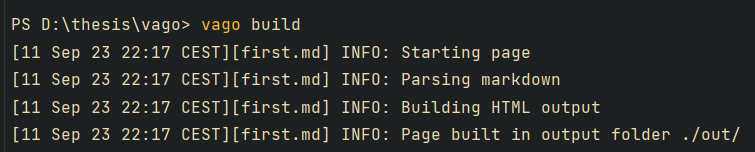
\includegraphics[width=1\textwidth]{/results/vagobuild}
    \caption{VaGo build execution with first.md}
    \label{fig:figure}
\end{figure}

Now, inspecting the \emph{/out/} folder, a new file can be seen with the same name as the input file, but with the
HTML extension: \emph{first.html}.
Reviewing the content of this file, it can be verified that it has been correctly parsed, as each token is correctly
mapped to its equivalent HTML tag (whole file not included for simplicity):

\begin{code}
<section>
<h2>
    Blockquotes</h2>
    <p><strong>This is bold text</strong></p>
    <p><strong>This is bold text</strong></p>
    <p><em>This is italic text</em></p>
    <p><em>This is italic text</em></p>
    <p><del>Strikethrough</del></p>

    </section>



    <section>
    <h2>Lists</h2>
    <blockquote>
    <p>Blockquotes can also be nested&hellip;</p>

    <blockquote>
    <p>&hellip;by using additional greater-than signs right next to each other&hellip;</p>

    <blockquote>
    <p>&hellip;or with spaces between arrows.</p>
    </blockquote>
    </blockquote>
    </blockquote>

    </section>



    <section>
    <h2>Code</h2>
    <p>Unordered</p>
    <ul>
    <li>Create a list by starting a line with <code>+</code>, <code>-</code>, or <code>*</code></li>
    <li>Sub-lists are made by indenting 2 spaces:

    <ul>
    <li>Marker character change forces new list start:

    <ul>
    <li>Ac tristique libero volutpat at</li>
    <li>Facilisis in pretium nisl aliquet</li>
    <li>Nulla volutpat aliquam velit</li>
    </ul></li>
    </ul></li>
    <li>Very easy!</li>
    </ul>
    <p>Ordered</p>
    <ol>
    <li><p>Lorem ipsum dolor sit amet</p></li>

    <li><p>Consectetur adipiscing elit</p></li>

    <li><p>Integer molestie lorem at massa</p></li>

    <li><p>You can use sequential numbers&hellip;</p></li>

    <li><p>&hellip;or keep all the numbers as <code>1.</code></p></li>
    </ol>
    <p>Start numbering with offset:</p>
    <ol>
    <li>foo</li>
    <li>bar</li>
    </ol>

    </section>



    <section>
    <h2>Tables</h2>
    <p>Inline <code>code</code></p>
    <p>Indented code</p>
    <pre><code>// Some comments
    line 1 of code
    line 2 of code
    line 3 of code
    </code></pre>
\end{code}


Nonetheless, in order to verify that it's working as expected with all the tags correctly set, it is imperative to test
it out in a browser, to determine if the content is being displayed as it should.
Therefore, this can be tried out by simply starting a server and accessing this file using URL path \emph{/first.html}.
On a side note, the home page is not being set in the configuration file, hence the server will lack of a homepage,
although it doesn't impose an issue for the purpose of this test.
The test can be started by using the command \emph{vago serve}:

\begin{figure}
    \centering
    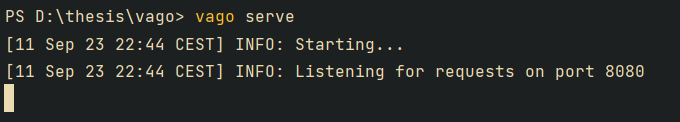
\includegraphics[width=1\textwidth]{/results/vagoserve}
    \caption{VaGo serve execution with first.md}
    \label{fig:serve}
\end{figure}


Then, accessing \emph{localhost:8080/first.html} the following page can be seen in the browser:

\begin{figure}
    \centering
    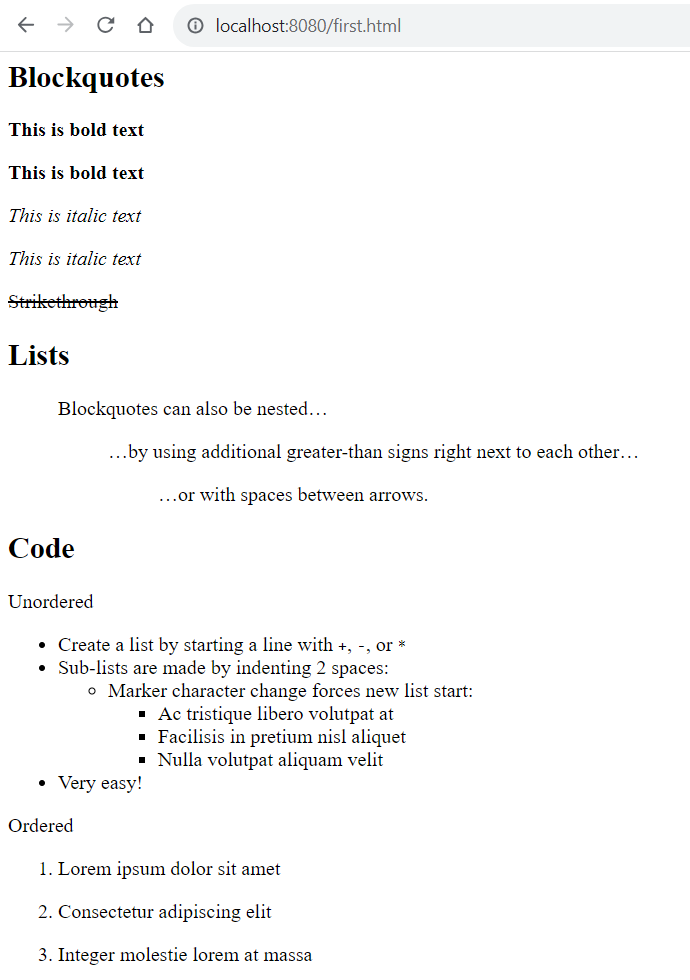
\includegraphics[width=0.8\textwidth]{/results/browserfirsthtml}
    \caption{first.html displayed in browser.}
    \label{fig:browserfirst}
\end{figure}

With this simple test, the main functionality of parsing, generating, serving and routing has been successfully
demonstrated, proving VaGo to be a static site generator capable of performing the most simple tasks.

Notwithstanding, there is left to try the templating and theming system, to ensure its flexibility capabilities.
For this, a new input file is constructed with several sections divided by titles.
The new file will be named as lorem.md, and it has the following structure (not all the content is displayed for
simplicity):

\begin{code}

    # Lorem Ipsum

    ## What is Lorem Ipsum?

    Lorem Ipsum is simply dummy text of the printing and
    typesetting industry. Lorem Ipsum has been the industry's
    standard    dummy text ever since the 1500s, when an
    unknown printer took a galley of type and scrambled it
    to make a type specimen book. It has survived not only
    five centuries, but also the leap into electronic
    typesetting, remaining essentially unchanged. It was
    popularised in the 1960s with the release of Letraset
    sheets containing Lorem Ipsum passages, and more
    recently with desktop publishing software like Aldus
    PageMaker including versions of Lorem Ipsum.

    ## Why do we use it?

    It is a long established fact that a reader will be
    distracted by the readable content of a page when
    looking at its layout. The point of using Lorem
    Ipsum is that it has a more-or-less normal
    distribution of letters, as opposed to using
    'Content here, content here', making it look like
    readable English. Many desktop publishing packages
    and web page editors now use Lorem Ipsum as their
    default model text, and a search for 'lorem ipsum'
    will uncover many web sites still in their infancy.
    Various versions have evolved over the years,
    sometimes by accident, sometimes on purpose
    (injected humour and the like).

\end{code}

Since the content of this new input file has defined sections, the previous template can be modified to take advantage
of this and provide a more customized structure, iterating over second headings \emph{H2} and using the same index to
iterate over \emph{P} values.
This is done by using the \emph{range} function from Go templates and storing a
reference to \emph{P} to avoid losing its content within the range context, then providing the same iterator
\emph{\$i} on the function \emph{index}.

These functionalities are all part of the native Go template system, so VaGo takes advantage of the extended already
provided features to provide flexible customization options.

\begin{code}
<!DOCTYPE html>
<html lang="en">
<head>
<meta charset="UTF-8">
<link rel="stylesheet" href="styles.css">
<title> {{ .H1 }} </title>
</head>
<body>

<h1> {{ .H1 }} </h1>
{{ $p := .P }}
{{
    range $i, $H2 := .H2 }}

<section>
<h2>{{ $ H2 }}</h2>
{{ index $p $i }}
</section>

{{ end }}

</body>
</html>
\end{code}

In the same way, a new CSS file is added to the \emph{/styles/} folder, making use of the theme variables that will be
defined later:

\begin{code}
section{
background-color: {{ .background }};
margin: {{ .margin }};
padding:  {{ .padding }};
}
\end{code}

Following this, the variables \emph{background, margin, padding} are defined in the \emph{theme.yaml} file, and
further users can modify these variables to match their styling needs. For the moment, the content of this file will
be the following:

\begin{code}
background: "#696969"
margin: "5px"
padding: "5px"
\end{code}

Consequently, a few modifications to the configuration file (config.yaml) are required to add the new theme, and the
new file \emph{lorem} is added as a homepage too, in order to try out the home page feature.

\begin{code}
input: "./source/"
template: "./template/index.html"
output: "./out/"

# Theme:
styles: "./styles/"
theme: "./theme.yaml"

home: "lorem.html"
\end{code}

Once everything is set up, a new building process can be started using the same command \emph{vago build}, and this
will provide context on the files parsed and created, including the style files.

\begin{figure}
\centering
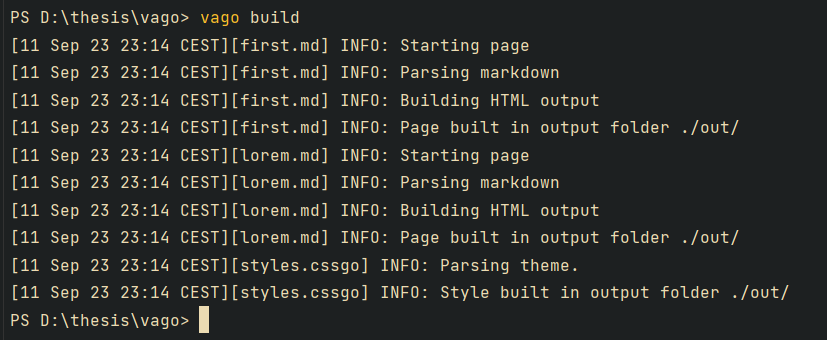
\includegraphics[width=1\textwidth]{/results/vagobuild2}
\caption{Building with new file, template and theme.}
\label{fig:build2}
\end{figure}

After this, the files \emph{lorem.html} and \emph{styles.css} has been added to the output folder \emph{/out/}.
Then, to verify the web content and its new styles added, a new server has to be started using the same command
\emph{vago serve} (output omitted for simplicity).
Following, the URL \emph{localhost:8080} is accessed, and the content of lorem.html is correctly displayed as home
page, with a set of styles provided as expected:

\begin{figure}
\centering
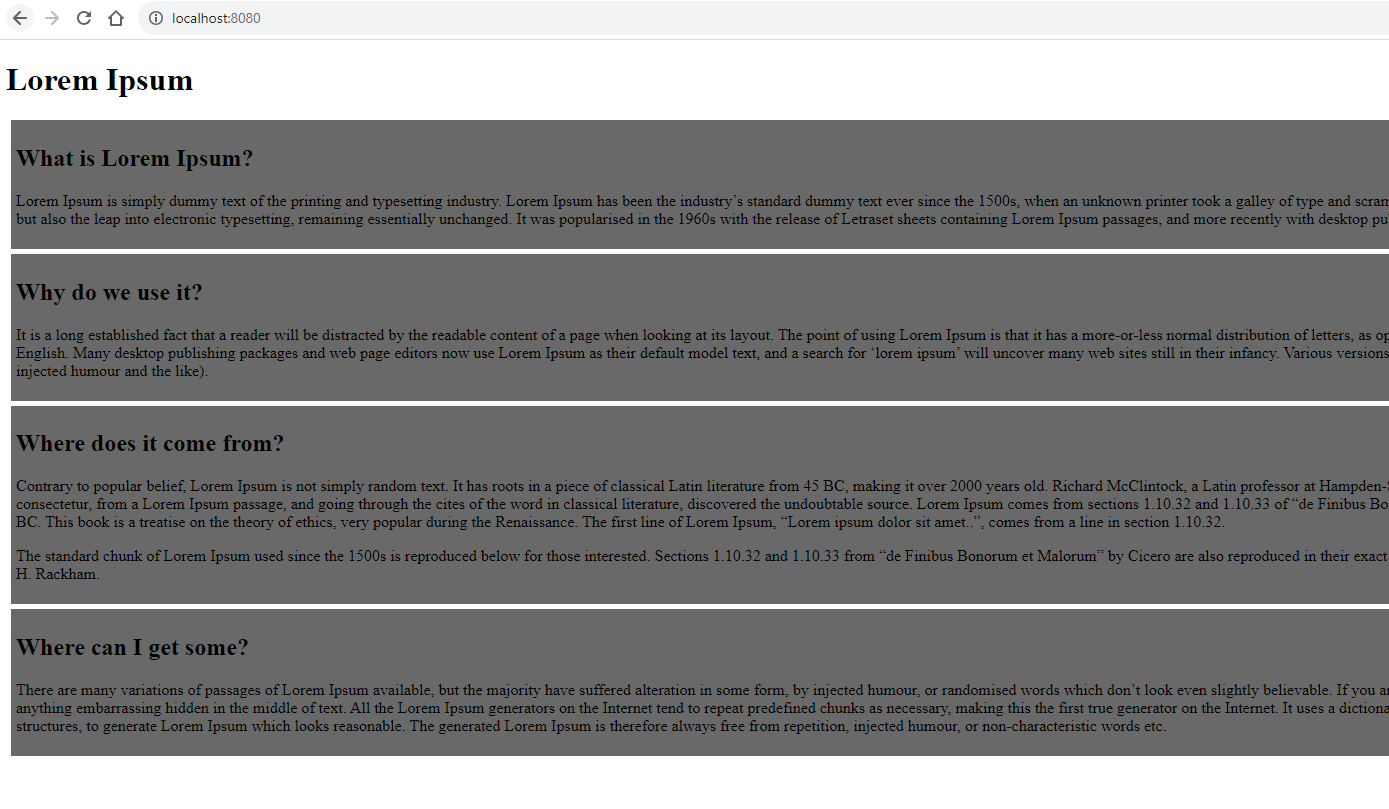
\includegraphics[width=1\textwidth]{/results/vagoserve2}
\caption{Serving lorem.html as homepage with styles.}
\label{fig:serve2}
\end{figure}

The provided color scheme and separation between sections may not be desirable. However, this can be easily modified
by accessing the theme file and adding the desired characteristics. A cyan like color should provide better
readability, and an increased margin and padding should be enough to split the sections.

\begin{code}
background: "#C0FFEE"
margin: "18px"
padding: "24px"
\end{code}

After building and starting the server once again (ouput omitted for simplicity), the following content is displayed in
the browser:

\begin{figure}
\centering
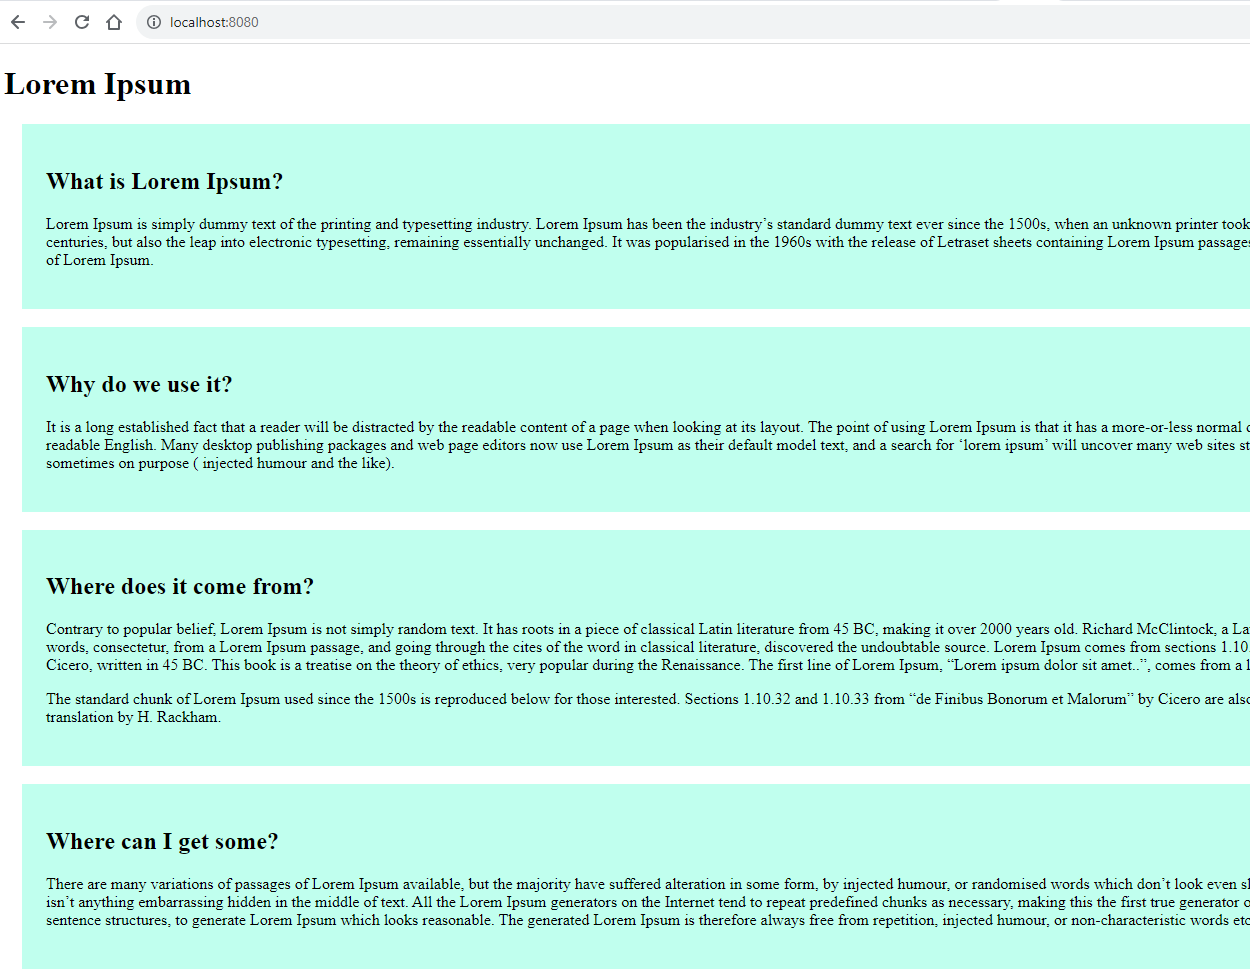
\includegraphics[width=1\textwidth]{/results/vagoserve3}
\caption{Serving lorem.html after modifying the theme.}
\label{fig:serve3}
\end{figure}

    % Conclusions
    %! Author = javif
%! Date = 9/12/2023


\chapter{Conclusion}\label{ch:conclusion}

As demonstrated on previous chapter, VaGo is a software capable of obtaining input markdown files from an established
folder, read each file content, navigate through the abstract syntax tree, obtain the required tokens to build up a
web page, parse it into respective HTML tags, create HTML files accordingly to the input content using the same name,
build up dedicated styles using a theme system reading customization variables, read configuration file to adapt
system to user specifications, provide a listener server on a provided port, route requests to map the same file name
convention to target URLs, display insightful logging and an intuitive command interface with discerning usage
documentation.


As a result, it has been shown that the implementation of VaGo successfully meets the requirements outlined in
previous sections.
Furthermore, it can be regarded as a favorable alternative to existing Static Site Generators, as
it possesses the ability to execute a majority of the characteristics commonly observed in the present market.
This is without accounting for some other measures that are not the primary emphasis of this project, such as its
lightning-quick creation and serving of files, which opens up new possibilities beyond merely serving static
information: The rapid pace of building construction facilitates the expansion of serverside rendering capabilities.


What's more, VaGo has been developed using a minimalistic approach, reducing the code and the cognitive load to the
lowest possible, with a balance between fulfilling requirements and following the proposed design with the desired
simplicity.
This minimalistic philosophy has demonstrated an overall increased productivity in terms of implementation, while
reducing the amount of complications and challenges to face when dealing with bugs and errors, with the addition of
being an open door to extension given that the code base is very simple and easy to read and understand, allowing
future collaborators to improve its functioning and/or add new features.

All in all, VaGo has been capable of meeting the requirements established at the beginning, following the minimalistic
approach, providing a fully functional static site generator.
Hence, this project serves as a proof that selecting the correct tools, frameworks, language, libraries and modules,
by setting a realistic set of requirements, with the right approach that ties up the development process without
limiting its creativity, and understanding the balance between proposed design and implementation changes, any software
project can be developed with ease, ending up with a robust, flexible and open to extension results.

From the point of view of users, VaGo is ready to be used for those looking for a simple software that can allow them
to focus on content creation rather than software development details.
Create markdown content, input a couple of commands and have your static file served site ready to go.


    % Future lines
    %! Author = javif
%! Date = 9/12/2023

\chapter{Future lines}\label{ch:futurelines}

Although VaGo is capable of performing the task evaluated in this project, it is far from perfect, as there are some
improvements and features that can be added as a static site generator.

For instance, the software requires the whole code to be in the same parent folder as the input and output content,
styles, template, configuration and more.
Thus, it would be very handy to have a feature that allows the creation of a new VaGo project folder from scratch,
only with the required folders and files needed to start crafting content, without the code being in the same
directory, as it would allow the creation of multiple projects with the same code folder in another place in the
system, allowing the user to have a separation of concerns between the content and VaGo code base, useful for further
arrangement and manipulation.

On the other hand, given that it uses the concept of themes for styling, a theme package manager can be created along
with the main project to provide extended capabilities for theme publication and sharing, as well as download and
install other themes.
This will allow the user to follow the philosophy of only focusing on content creation and theme customization, as it
would subtract the need of crafting CSS styles files from scratch.

Finally, in order to meet the current state of the art of the most popular static site generators, VaGo must have the
capability of extending its functionalities via plugins, which must be easy to find, install, use and manage.
An example of a handy plugin, is the capability of adding LaTeX-like content writing, allowing the user to not only
create files on markdown format, but also extending these to use LaTex nomenclature, which is useful for
mathematicians as they can easily compose complex formulas.
This would require a plugin manager, to navigate through existing plugins and install them on command.

    % Bibliography
%    \markdownInput{chapters/bibliography.md}

    \bibliography{chapters/citations}
    \bibliographystyle{sapthesis}

\end{document}
